\begin{definition}[Parallelotop]
    Seien $a_1, \ldots, a_d \in \mathbb{R}^n \ (d \leq n)$ Dann nennen wir
    \begin{equation*}
    	P \left( a_1, \ldots, a_d \right) \coloneqq 
    	\left\lbrace 
    	\sum\limits_{j=1}^n t_j a_j | t_j \in [0,1], j = 1, \ldots, d    
    	\right\rbrace
    \end{equation*}
    das von $a_1, \ldots, a_d $ augespannte \textbf{Parallelotop} (manchmal auch d-Spat).
\end{definition}

An dieser Stelle ein kleiner Einschub: Eine allgemeinere Theorie für d-dimensionale Inhalte liefert das sogenannte
Hausdorff-Maß $\mathcal{H}^d$. Dieses ist jedoch sehr viel abstrakter und schwierig 
'auszurechnen'. Mithilfe von Mannigfaltgkeiten kommt man schneller zu Ergebnissen. \\
Aus der theoretischen Physik ist uns bereits das Maß über die Delta-Distribution bekannt, mit dem wir zum Beispiel die Ladungsdichte einer Punktmasse 
\begin{equation*}
\rho(r)=\int\limits_{\mathbb{R}^3}q\delta(r-r_o)\mathrm{d}V
\end{equation*}
exakt definieren können. 
\newpage
\begin{satz}
    \mbox{}
    Seien $a_1, \ldots, a_n \in \mathbb{R}^n$ und $v(a_1, \ldots , a_n) \coloneqq \mathcal{L}^n (P (a_1, \ldots, a_n))$ das von ihnen aufgespannte Volumen. Dann gilt:
    \begin{enumerate}
        \item[i)]
            $v(a_1, \ldots, \lambda a_k, \ldots, a_n) = 
            |\lambda| v(a_1, \ldots, a_n) \forall \lambda \in \mathbb{R}^n $
        \item[ii)]
            $v(a_1, \ldots, a_k + a_j, \ldots, a_n) = v(a_1, \ldots, a_n) $
            falls $k \neq j $ \\
            \linebreak
            Dies ist bekannt als \emph{Prinzip des Cavaleri}. Als Veranschaulichung kann
            ein Stapel Spielkarten dienen: Egal wie man eine Seitenfläche von einem Rechteck
            in ein Parallelogramm (oder umgekehrt) verschiebt, 
            das Volumen des Stapels bleibt gleich. \\
            \begin{center}
            	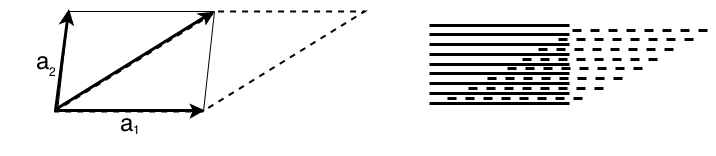
\includegraphics[scale=0.5]{pictures/004-01.png}
            \end{center}
        \item[iii)]
            $v(a_1, \ldots, a_n) = 1 $ falls $a_1, \ldots, a_n $ ein Orthonormalsystem
            in $\mathbb{R}^n $ bilden. \\
            (Der Parallelotop ist dann der Einheitswürfel.)
        \item[iv)]
            $v(a_1, \ldots, a_n) = |\det A|$ für $A \coloneqq (a_1 | \ldots | a_n) $ \\
            \linebreak
            Das heißt die Determinante der Matrix mit den Spaltenvektoren $a_1, \ldots, a_n$
            liefert das Volumen des aufgespannten Parallelotops. (Vgl. lin. Algbebra)
    \end{enumerate}
\end{satz}

    Es ist zu beachten, dass die Eigenschaften i) - iii) bereits iv) implizieren. Die Argumentation
    dazu verläuft wie zu den aus der Linearen Algebra bekannten Eigenschaften der Determinante, vgl.
    auch die axiomatische Definition der Determinante.
\newpage
\begin{proof}
    \mbox{}
    \begin{enumerate}
        \item[a)] 
            Nehmen wir an, $a_1, \ldots, a_n$ sind linear abhängig. \\
            Dann ist das aufgespannte Parallelotop 'flach', da es in mindestens 
            einer Dimension an Ausdehnung fehlt und somit
            $v(a_1, \ldots, a_n) = 0 $. Weil die Determinante jeder singulären Matrix verschwindet, ist iv) korrekt. Es folgt sofort, dass auch i) und ii) richtig sein müssen.
        \item[b)]
            Nun seien $a_1, \ldots, a_n$ linear unabhängig. \\
            Sei $\lbrace e_1, \ldots, e_n \rbrace$ die Standard-Orthonormalbasis in
            $\mathbb{R}^n $. Für diese gilt iii) nach der Definition des Lebesgue-Maß. Sie bildet nämlich einen Quader der Kantenlänge Eins. \\
            Weiter seien nun $U \coloneqq P(e_1, \ldots, e_n),\
            V \coloneqq P(a_1, \ldots, a_n) $ \\
            Dann ist $A: \mathrm{int}\ U \rightarrow \mathrm{int}\ V $
            ein Diffeomorphismus (A ist regulär, ist damit differenzierbar und
            besitzt ein differenzierbares Inverses). \\
            Offenbar ist $A'(y) = A \ \ \ \forall y $ \\
            Wenn wir nun den Transformationssatz (Kap. 24) an, so ergibt sich
            \begin{equation*}
            	\mathcal{L}^n (V) = \int\limits_V \mathrm{d}x \stackrel{y = Ax}{=}
            	\int\limits_U |\det A| \mathrm{d}y = |\det A| \underbrace{\mathcal{L}^n (U)}_1
           		 = |\det A|
           	\end{equation*}
            Daraus folgt iv) und i), ii), iii) als Eigenschaften
            der Determinanten
    \end{enumerate}
\end{proof}

Machen wir uns noch einmal die Zielstellung klar. Wir wollen den d-dimensionalen Inhalts
$v_d (P(a_1, \ldots, a_d))$ im $\mathbb{R}^n $ bestimmen.\\
Dabei ist folgende Idee zweckmäßig: Man betrachtet $P(a_1, \ldots, a_n)$ als Teilmenge eines d-dimensionalen
Vektorraums $X$ und nimmt das d-dimensional Lebesgue-Maß in $X$.\\
Somit sollte 
\begin{equation*}
	v_d: 
	\underbrace{\mathbb{R}^n \times \ldots \times \mathbb{R}^n }_{\text{d-mal}}
	\rightarrow \mathbb{R}_{\geq 0}
\end{equation*}
folgende Eigenschaften haben:
\begin{enumerate}
    \item[(v1)]
        $v_d (a_1, \ldots, \lambda a_k, \ldots, a_d) = |\lambda| v_d(a_1, \ldots, a_d)
        \forall \lambda \in \mathbb{R} $
    \item[(v2)]
        $v_d (a_1, \ldots, a_k + a_j, \ldots, a_d) = v_d(a_1, \ldots, a_d) $
        falls $k \neq j$ (Prinzip des Cavaleri)
    \item[(v3)]
        $v_d(a_1, \ldots, a_d) = 1 $ falls $\lbrace a_1, \ldots, a_d \rbrace $
        orthonormal zueinander sind.
\end{enumerate}
\newpage
\begin{satz}
    $v_d$ ist durch (v1), (v2), (v3) eindeutig bestimmt, und es gilt:
    \begin{equation}
        v_d(a_1, \ldots, a_d) = 
        \sqrt[]{\det \underbrace{A^T A}_{\in \mathbb{R}^{d \times d}}}
        \text{ mit } 
        A \coloneqq\underbrace{(a_1 | \ldots | a_d)}_{\in \mathbb{R}^{n \times d}}
    \end{equation}
\end{satz}
An dieser Stelle können wir sofort einige Aussagen treffen:\\
\begin{enumerate}
    \item
        für $d=n $ liefert (30.1) Gleichung iv) in Satz 1
    \item
        $A^T A $ ist stets symmetrisch und positiv definit
        $\left( \scap{x}{A^T Ax}=
        \scap{Ax}{Ax}= \|Ax\|^2 \geq 0 \right)$
        und somit ist auch stets $\det\ A^T A \geq 0 $
    \item
        $v_d (a_1, \ldots, a_d)$ verschwindet genau dann, wenn $a_1, \ldots, a_d$ linear abhängig sind.
\end{enumerate}

\begin{proof}
    Dies ist für das Selbststudium überlassen. Es lohnt sich jedoch
	\begin{equation*}
		A^T A = 
    	\begin{pmatrix}
        	\alpha_{11} & \ldots & \alpha_{1n} \\
        	\vdots      & \ddots & \vdots \\
        	\alpha_{n1} & \ldots & \alpha_{nn}
    	\end{pmatrix}\
   		 \text{mit\ } \alpha_{ij}=\scap{a_i}{a_j}
	\end{equation*}	    
    zu verwenden und wie bei den Eigenschaften der Determinante zu argumentieren.
\end{proof}

\begin{beispiel}
    $d = n-1 $: Sei $a_1, \ldots, a_{n-a} \in \mathbb{R}^n, 
    a \coloneqq a_1 \wedge \ldots \wedge a_{n-1} $
    \begin{equation}
        v_{n-1} (a_1, \ldots, a_{n-1}) = |a|_2
    \end{equation}
    Die euklidische Länge des äußeren Produkts liefert also das Volumen.\\
    Das prüfen wir leicht nach: 
    \begin{equation*}
    	\begin{pmatrix}
        a^T \\
        \rule[.5ex]{1em}{1pt}\\
        A^T
    \end{pmatrix}
    \bullet
    \begin{pmatrix}
        a & | & A 
    \end{pmatrix}
    =
    \begin{pmatrix}
        \scap{a}{a} & 0 \\
        0 & A^T A
    \end{pmatrix}
    \end{equation*}
    
    denn $\scap{a_i}{a_j} = 0 \ \ \ \forall j $ mit $A$ wie in (1). Es folgt sofort
	\begin{equation*}
	||a||_2^2 \cdot \det A^T A = (\det (a|A))^2 \stackrel{(29.4)}{=}
    ||a||_2^4
	\end{equation*}	    
    und dann mit (1) sofort (2).
\end{beispiel}

Es stellt sich folgende Frage: Existiert für eine Mannigfaltigkeit $M$ eine Transforamtion, so dass das
Volumen eines Quaders $Q \in \mathbb{R}^d $ auf das eines Parallelotops 
$P \subset T_uM \in \mathbb{R}^n $ abgebildet wird? Dass also
\begin{equation*}
v_d(\textbf{Quader }Q) \xrightarrow{\varphi'(x)} v_d(\textbf{Parallelotop } P)
\end{equation*}
\begin{center}
	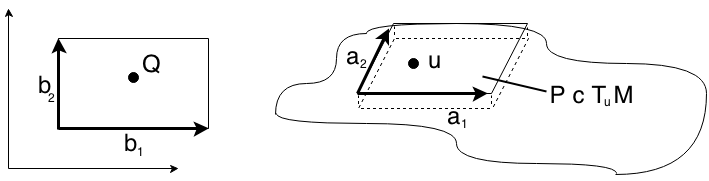
\includegraphics[scale=.5]{pictures/004-02.png}
\end{center}
Für einen Quader $Q = P(b_1, \ldots, b_d) \subset \mathbb{R}^d $ ist 
$P(a_1, \ldots, a_d) \subset T_uM \in \mathbb{R}^n $ das zugehörige Parallelotop, falls
$a_j = \varphi'(x) b_j $,für $ j=1, \ldots, d $

\begin{satz}
    Sei $M$ eine d-dimensionale Mannigfaltigkeit, $\varphi$ eine Parametrisierung um $\varphi(x) = u \in M $
    und $Q \coloneqq P(b_1, \ldots, b_d) \subset \mathbb{R}^d $ ein Quader mit $b_j \in \mathbb{R}^d$, weiterhin sei $a_j \coloneqq \varphi'(x) b_j,\ j= 1, \ldots, d $ \\
    Dann gilt:
    \begin{equation}
        v_d(a_1, \ldots, a_d) = 
        \sqrt{\det \varphi'(x)^T \varphi'(x)}\ v_d(b_1, \ldots, b_d)
    \end{equation}
\end{satz}

\begin{definition}[Maßtensor] Das Produkt der transponierten Ableitung mit sich selbst
	\begin{equation*}
		\varphi'(x)^T \varphi'(x) \in \mathbb{R}^{d \times d}
	\end{equation*}
    heißt \textbf{Maßtensor}    von $\varphi$ in $x$, dessen Determinante
    \begin{equation*}
		g^\varphi (x) \coloneqq \det \varphi'(x)^T \varphi'(x)
	\end{equation*}
    man die \textbf{Gramsche Determinante} von $\varphi$ in $x$ nennt.
\end{definition}
\newpage
\begin{proof}
    Sei $B = (b_1, \ldots, b_d) \in \mathbb{R}^{d \times d}$ und 
    $A = (a_1, \ldots, a_d) \in \mathbb{R}^{n \times d}$. Mit Gleichung (30.1) folgt
	\begin{equation*}
		v_d(a_1, \ldots, a_d) 
    	= \sqrt{\det A^T A} = \sqrt{\det ((\varphi'(x) B)^T \varphi'(x) B)}
   		= \sqrt{\det \varphi'(x)^T \varphi'(x)} 
   		\underbrace{\sqrt{\det B^T B}}_{= v_d(b_1, \ldots, b_d)}
	\end{equation*}	    
\end{proof}

Sei nun $M \subset \mathbb{R}^n $ eine d-dimensionale Mannigfaltigkeit,
$\varphi: V \rightarrow U $ eine lokale Parametriesierung,
$f: \rightarrow \mathbb{R} $ eine Funktion auf dem Kartengebiet $U$.\\
Motiviert durch die Riemann-Summen (Kap. 22)\\
$\sum f(u_i) v_d(P_i) = \sum f(\varphi(x_i)) \sqrt{g^\varphi (x_i)} v_d(Q_i) $
mit $P_i = \varphi'(x_i) Q_i $
definieren wir:

\begin{definition}[Integral über über Kartengebiet]
    \begin{equation}
        \int\limits_U f \mathrm{d}a 
        \coloneqq \int\limits_V f(\varphi(x)) \sqrt{g^\varphi (x)} \mathrm{d}x
    \end{equation}
    als \textbf{Integral von $f$} über das Kartengebiet $U$ falls die rechte
    Seite existiert.\\
    $f$ heißt dann \textbf{integrierbar} auf $U$.
\end{definition}

\textbf{Bemerkung:}
\begin{enumerate}
    \item[-]
        die rechte Seite in (30.4) ist ein Lebesgue-Integral in $\mathbb{R}$
    \item[-]
        damit die Definition von (30.4) sinnvoll ist, sollte die rechte Seite
        unabhängig von $\varphi$ sein
    \item[-]
        mittels des Hausdorff-Maß $\mathcal{H}^d $ kann
        $\int\limits_U f \mathrm{d}a $
        völlig analog zum Lebesgue-Maß definiert werden
        $\left(\int\limits_U f(u) \mathrm{d} \mathcal{H} (u) \right) $
    \item[-]
        für n-dimensionale Mannigfaltigkeiten $M \subset \mathbb{R}^n: \\
        \int\limits_U f \mathrm{d}a = $ Lebesgue-Integral 
        $\int\limits_U f \mathrm{d}x $ falls dieses existiert
\end{enumerate}
\newpage
\begin{satz}
    Sei $M \subset \mathbb{R}^n $ eine d-dimensionale Mannigfaltigkeit,\\
    $U \subset M $ ein Kartengebiet, $f:U \rightarrow \mathbb{R} $ und
    $\varphi_i: V_i \rightarrow U,\ i=1,2 $ seien zugehörige Parametrisierungen. Dann gilt
    \begin{equation*}
    	\int\limits_{V_1} f(\varphi_1(x)) \sqrt{g^{\varphi_1} (x)} \mathrm{d}x
    	= \int\limits_{V_2} f(\varphi_2(x)) \sqrt{g^{\varphi_2} (x)} \mathrm{d}x
    \end{equation*}
   	falls eines der Integrale existiert.
\end{satz}

(30.4) ist also unabhängig von der Parametrisierung. Denn
\begin{equation}
    f(.) \text{ int'bar auf } U
    \Longleftrightarrow f(\varphi(.)) \sqrt{g^\varphi (x)} 
    \text{ int'bar auf } V
    \text{ für eine Param. }
    \varphi: V \rightarrow U
\end{equation}

\begin{proof}
    $\psi \coloneqq \varphi_1^{-1} \bullet \varphi_2: V_2 \rightarrow V_1 $
    ist ein Diffeomorphismus nach Lemma 5. Wir wenden wieder den Transformationssatz an und erhalten
	\begin{equation*}
		\int\limits_{V_1} f(\varphi_1(x)) \sqrt{g^{\varphi_1} (x)} \mathrm{d}x
    	\stackrel{x=\psi(y)}{=}
   	 	\int\limits_{V_2} f(\varphi_1(\psi(y)))
    	\underbrace{
        \sqrt{\det \varphi_1'(\psi(y))^T \varphi_1'(\psi(y))}
        \underbrace{
            |\det \psi'(y)|
            }_{
            = \sqrt{\det \psi'(y)^T \psi'(y)}}
        }_{
        = \sqrt{\det \psi'^T \varphi_1'^T \psi' \varphi_1'}
        = \sqrt{\det (\psi' \varphi_1')^T \psi' \varphi_1'}
        }
    	\mathrm{d}y
	\end{equation*}	    
    denn da
    \begin{equation*}
		\varphi_2 (y) = \varphi_1 (\psi(y))
	\end{equation*}	   
	folgt mit Kettenregel
	 \begin{equation*}
    	\varphi_2' (y) = \varphi_1' (\psi(y)) \psi'(y)
	\end{equation*}	 
	und somit die Behauptung.
\end{proof}